\chapter{Title of Chapter 1}

\section{Introduction}

Text of introduction.

\section{Section 2}

Example of equation of a given parameter P as described in \cite{Author2020}, which is defined by the ratio of the peak value $V_{\text{peak}}$ and the average value $V_{\text{avg}}$ as:
\begin{equation}
	\label{P}
	\text{P}_{\text{v}}=10\log\left( \frac{\text{V}_{\text{peak}}}{\text{V}_{\text{avg}}} \right)
\end{equation}

The reference to the equation is \eqref{P}.

Figure \ref{bird_jpeg} presents a bird in JPEG format.

\begin{figure}[!h]
	\centering
	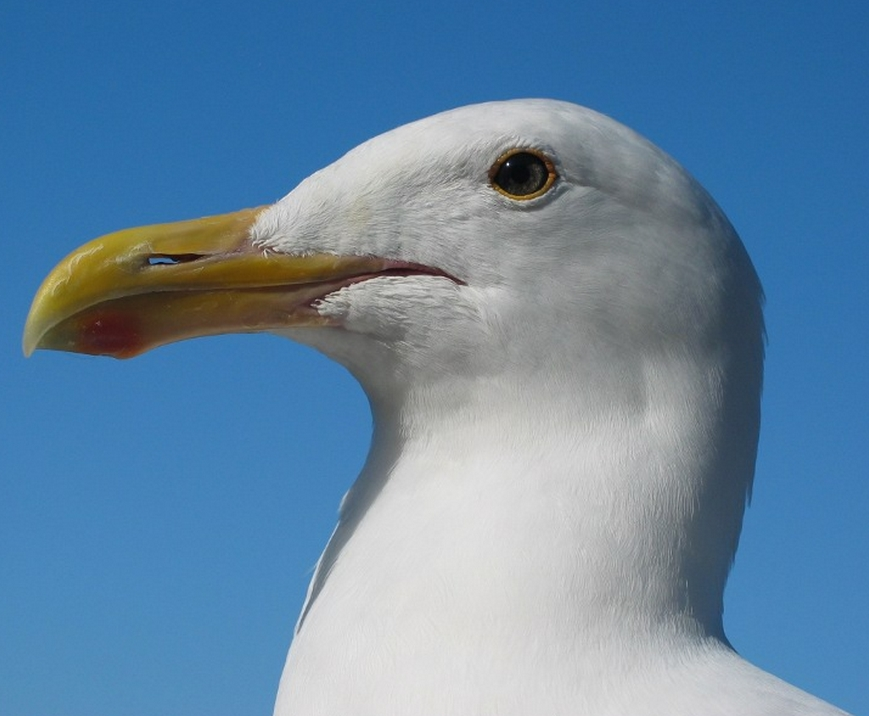
\includegraphics[width=0.75\textwidth,]{Figures_Chapter_1/bird.jpg}
	\caption{Bird in JPEG format}
	\label{bird_jpeg}
\end{figure}

The PDF format can also be used in Figure \ref{bird_pdf}

\begin{figure}[!h]
	\centering
	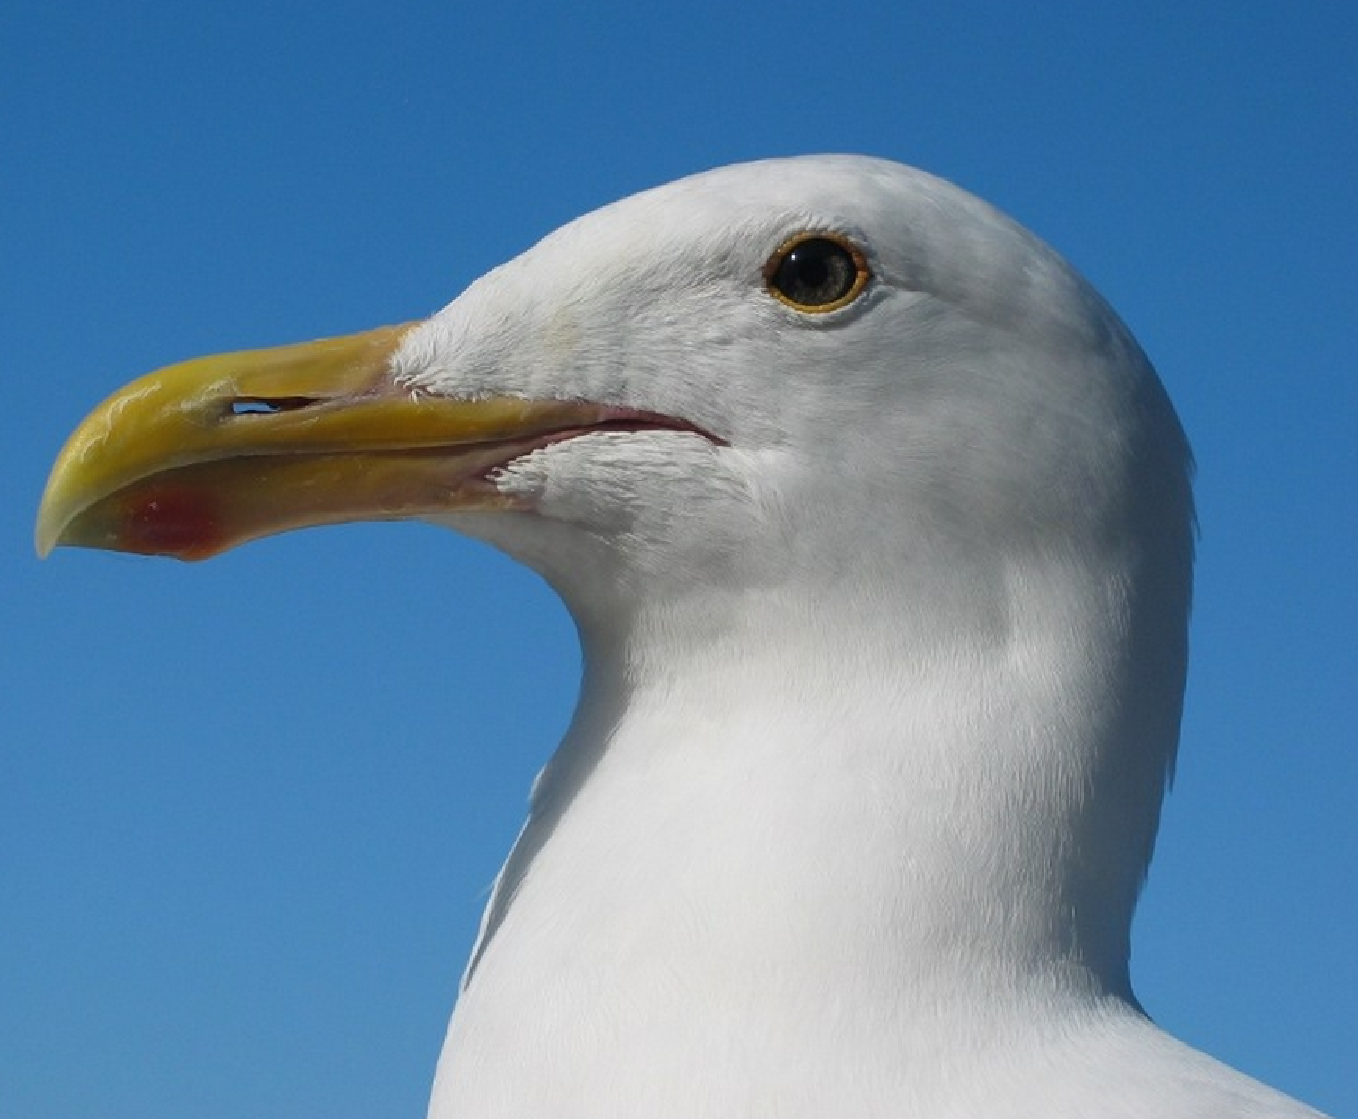
\includegraphics[width=0.75\textwidth,]{Figures_Chapter_1/bird.pdf}
	\caption{Bird in JPEG format}
	\label{bird_pdf}
\end{figure}

\section{Conclusion}

This chapter has provided an overview of the X ...

The main contributions of these dissertations are thoroughly presented in the following chapters.